Met de moderne SSDs is defragmentation niet meer nodig, sterker het zou je SSD sneller kunnen doen verouderen. Als je nog een harddisk gebruikt legt deze sectie je uit wat defragmentation is en waarom je het nodig hebt.

Defragmentatie is het netjes achter elkaar leggen van sectoren die behoren bij een bestand. Een harddisk is ingedeeld in sectoren (van bijv. 512 bytes). Elk bestand wordt opgehak in stukjes die in een sector passen en dan weggeschreven. Het filesystem houdt in een tabel bij welke sectoren er bij welk bestand horen en in welke volgorde ze gelezen moeten worden. Ideaal is het als alle data netjes op een cylinder ligt en alle sectoren netjes naast elkaar. Dan hoeft de leeskop het minst te bewegen en kan er de maximale hoeveelheid data gelezen worden.

Tijdens het gebruik van een harddisk worden er bestanden geschreven, verwijderd en bestanden worden groter of kleiner. Dit betekent dat data niet altijd meer op de ideale plek op de harddisk terecht komt. Als een bestand bijvoorbeeld groter wordt kan het zijn dat de eerste 100k keurig op de harddisk ligt maar dat de laatste 50k verspreid is geraakt over verschillende sectoren/cylinders. Dit heet fragmentatie.

Bij defragmentatie wordt de data weer op de ideale manier over de harddisk verspreid, waardoor er snelheidswinst bereikt kan worden. Defragmentatie is niet een eenmalige handeling, deze moet regelmatig herhaald worden.

\begin{minipage}[t]{\linewidth}
\raggedright
\adjustbox{valign=t}{%
   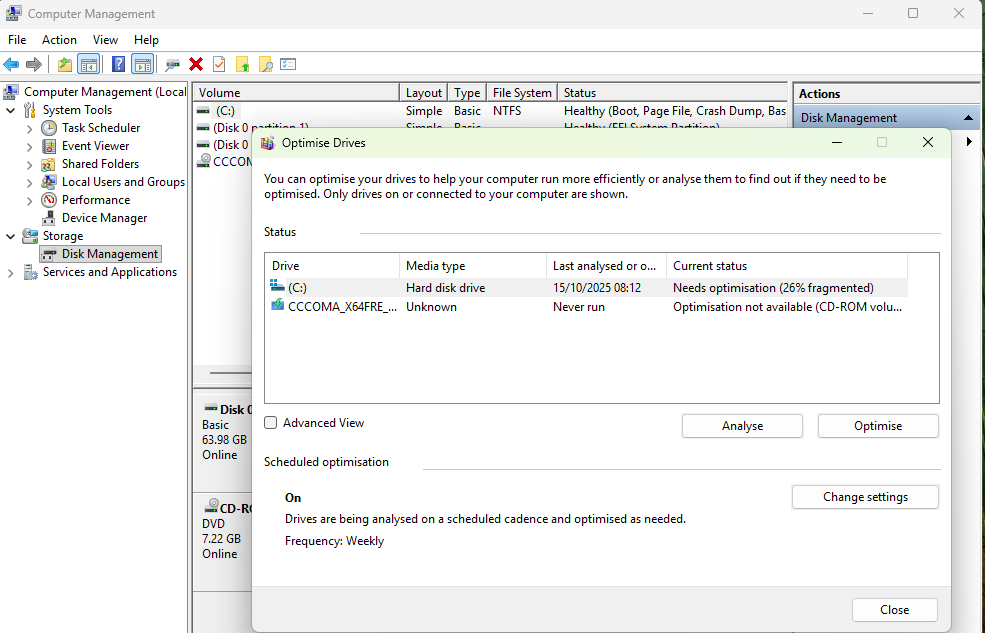
\includegraphics[width=0.99\linewidth]{computer_management-disks_defrag.png}%
}
\end{minipage}

SSDs hoeven niet gedefragmenteerd te worden omdat de toegang tot een SSD overal even snel is. Er is geen kop die verplaatst moet worden, dus je wint niets bij het defragmenteren. In het ergste geval wordt data ergens anders op de SSD weggeschreven en dat kost write-cycles wat slecht is voor een SSD.

